\documentclass[11pt,a4paper]{article}
%\documentclass[11pt,a4paper,draft]{book}
\usepackage[inner=3cm,textwidth=16cm,top=2.5cm,bottom=2.5cm]{geometry}
\usepackage[utf8]{inputenc}
\usepackage{lmodern}
\usepackage[T1]{fontenc}
% \usepackage[numbers]{natbib}
\usepackage[mode=buildmissing]{standalone}
\usepackage{tikz}
\usepackage{float}
%\usepackage{placeins}
%\usepackage{refcheck}
\usepackage{graphicx}
\usepackage{hyperref}
\usepackage{subcaption}
\usepackage{minted}
\usepackage{booktabs}
\usepackage{csquotes}
\usepackage{multirow}
\usepackage{tabularx}
\usepackage{tikz-uml}
\usepackage{threeparttable}
\usepackage[]{siunitx}
\usepackage{makecell}
\usepackage{graphbox}
\usepackage{diagbox}
\usepackage[draft]{fixme}
\usepackage{makecell}
%\usepackage{bibentry}
\usepackage{amsfonts}
\usepackage{amssymb}
\usepackage{amsmath}
\usepackage{mathabx}
\usepackage{cleveref}
\usepackage{datetime}
%\usepackage{svg}
\usepackage{lettrine}
%\usepackage{wrapfig}
%\usepackage[backend=biber,style=alphabetic,sorting=ynt]{biblatex}
%\usepackage[backend=biber,sorting=ynt,style=numeric]{biblatex}
%\usepackage[backend=biber,sorting=ynt,style=draft,backref=true]{biblatex}
\usepackage[backend=biber,
            defernumbers=true,
            sorting=ynt,
            style=numeric,
            %style=draft,
            backref=true]{biblatex}


\addbibresource{bibliography.bib}

% This allows for an additional line-breaking pass with the amount of
% "tolerable" white space per line increased by 1em.
% Needed for overfull hbox in bibliography
% \emergencystretch=1em
\usepackage[final]{microtype}

\usepackage[section]{placeins}

\usepackage{epstopdf}
\epstopdfDeclareGraphicsRule{.tif}{png}{.png}{convert #1 \OutputFile}
\AppendGraphicsExtensions{.tif}

\usepackage{pifont}
\newcommand{\cmark}{\ding{51}}%
\newcommand{\xmark}{\ding{55}}%
\newcommand{\eqmark}{{\bf \(\approx\)}}

\newcommand{\eg}{e.g.}
\newcommand{\ie}{i.e.}
\newcommand{\cf}{cf.}
\newcommand{\vs}{vs.}
\newcommand{\pros}{pros.}
\newcommand{\cons}{cons.}

\definecolor{lightgray}{rgb}{0.83, 0.83, 0.83}
\definecolor{lightblue}{rgb}{0.68, 0.85, 0.9}
\definecolor{lightgreen}{rgb}{0.56, 0.93, 0.56}
\definecolor{thistle}{rgb}{0.85, 0.75, 0.85}

\newcommand{\FIXME}[1]{{\color{red}#1}}
\newcommand{\PLAGIAT}[1]{{\color{magenta}#1}}

% Reset chapter number after each part
% \makeatletter
% \@addtoreset{chapter}{part}
% \makeatother

%\renewcommand{\baselinestretch}{1}

\usetikzlibrary{3d,calc,positioning}
\tikzumlset{font=\scriptsize\tt}
\setminted{fontsize=\scriptsize}

\renewcommand\UrlFont{\color{blue}\rmfamily}

% % % % % % % % % % % % % % % % % % % % % % % % % % % % % % % % % % % % % % % %
%    Page de garde (flyleaf.tex)   %
% % % % % % % % % % % % % % % % % % % % % % % % % % % % % % % % % % % % % % % %
% Dorian Depriester, 2014

\makeatletter
\def\@school{school}
\newcommand{\school}[1]{
  \def\@school{#1}
}

\def\@speciality{Speciality}
\newcommand{\speciality}[1]{
  \def\@speciality{#1}
}

\def\@ED{Doctoral School}
\newcommand{\ED}[1]{
  \def\@ED{#1}
}
\def\@address{Address}
\newcommand{\address}[1]{
  \def\@address{#1}
}

\def\@director{Director}
\newcommand{\director}[1]{
  \def\@director{#1}
}

\def\@advisor{Advisor}
\newcommand{\advisor}[1]{
  \def\@advisor{#1}
}
\def\@jurya{}{}{}
\newcommand{\jurya}[3]{
  \def\@jurya{#1,	& #2	& #3\\}
}
\def\@juryb{}{}{}
\newcommand{\juryb}[3]{
  \def\@juryb{#1,	& #2	& #3\\}
}
\def\@juryc{}{}{}
\newcommand{\juryc}[3]{
  \def\@juryc{#1,	& #2	& #3\\}
}
\def\@juryd{}{}{}
\newcommand{\juryd}[3]{
  \def\@juryd{#1,	& #2	& #3\\}
}
\def\@jurye{}{}{}
\newcommand{\jurye}[3]{
  \def\@jurye{#1,	& #2	& #3\\}
}
\def\@juryf{}{}{}
\newcommand{\juryf}[3]{
  \def\@juryf{#1,	& #2	& #3\\}
}
\def\@juryg{}{}{}
\newcommand{\juryg}[3]{
  \def\@juryg{#1,	& #2	& #3\\}
}
\def\@juryh{}{}{}
\newcommand{\juryh}[3]{
  \def\@juryh{#1,	& #2	& #3\\}
}
\def\@juryi{}{}{}
\newcommand{\juryi}[3]{
  \def\@juryi{#1,	& #2	& #3\\}
}
\makeatother

\makeatletter
\newcommand{\flyleaf}{
  \newgeometry{top=2.5cm, bottom=2.5cm, left=2cm, right=1cm}
  \begin{titlepage}
    \centering
    
\includegraphics[width=0.2\textwidth]{../images/EDITE.png}
    \hfill
    
\includegraphics[width=0.2\textwidth]{../images/epita.pdf}
    \hfill
    
\includegraphics[width=0.2\textwidth]{../images/lrde-big.png}\\
    \vspace{1cm}
    {\Large \@ED}\\
    \vspace{1cm}
    {\huge \bfseries{Doctoral Thesis}}\\
    \vspace{1cm}
    {\bfseries submitted to fullfil requirements for the degree of Doctor of}\\
    \vspace{0.5cm}
    
\includegraphics[width=0.3\textwidth]{../images/Logo_of_Sorbonne_University.pdf}\\
    %{\huge\bfseries \@school}\\
    \vspace{0.5cm}
    {\Large{\bfseries with the Doctoral Speciality of ``\@speciality''}}\\
    \vspace{1cm}
    {\LARGE \bfseries{\@title}} \\
    \vspace{1cm}
    \textit{presented and defended to the public by}\\
    \vspace{0.5cm}
    {\Large {\bfseries \@author}} \\
    \vspace{0.2cm}
    on the \@date \\
    \textit{before distinguished members of the jury}\\
    \vspace{0.2cm}
    \begin{tabular}{>{\bfseries}lll}
      \large Jury \\
      \@jurya
      \@juryb
      \@juryc
      \@juryd
      \@jurye
      \@juryf
      \@juryg
      \@juryh
      \@juryi
    \end{tabular}
    \vfill
    Director: {\bfseries \@director}\\
    Advisor: {\bfseries \@advisor}\\
    \vfill
    \@address
  \end{titlepage}

  \restoregeometry
}



\begin{document}
%
\flyleaf

\clearpage

		%Please consider the following section of the "Formvorschriften für die gedruckte Version"
	%Im Anhang ist eine Zusammenfassung (Abstract) mitzubinden. 
	%Ist die Arbeit in einer Fremdsprache verfasst, ist im Anhang jedenfalls eine deutsche Zusammenfassung mitzubinden.
\chapter{Abstract}
		This \LaTeX{} template provides example on how to format and display text, 
		mathematical formulas, and insert tables or images. There is a lot more you 
		can do with \LaTeX{}, for more information check out https://en.wikibooks.org/wiki/LaTeX.


\clearpage

\section{R\'{e}sum\'{e} long}
\subsection*{Introduction}


De nos jours, la \emph{Vision par ordinateur} et le \emph{Traitement d'Image (PI)} sont omniprésents dans la vie
quotidienne des gens. Il est présent à chaque fois que nous passons devant une caméra de vidéosurveillance, à chaque
fois que nous allons à l'hôpital faire une IRM, à chaque fois que nous conduisons notre voiture et passons devant un
radar et à chaque fois que nous utilisons notre ordinateur, smartphone ou tablette. Il ne peut plus être évité. Les
systèmes utilisant cette technologie sont parfois simples et parfois plus complexes. Aussi, l'usage qui est fait de
cette technologie a de nombreuses finalités telles que l'observation spatiale, le médical, l'amélioration de la qualité
de vie, la surveillance, le contrôle, les systèmes autonome, etc. Désormais, le \emph{Traitement d'images} dispose d'un
large éventail de sujets de recherches et malgré une masse de travaux antérieurs déjà contribués très importante, il
reste encore beaucoup à explorer.

Prenons l'exemple d'une application smartphone moderne qui propose une reconnaissance faciale afin de reconnaître les
personnes qui figurent dans d'une photo. Pour fournir un résultat précis, cette application devra faire beaucoup de
traitements différents en plusieurs étapes. De plus, il y a beaucoup de variables à gérer. Nous pouvons énumérer (non
exhaustivement) la météo, l'exposition lumineuse, la résolution, l'orientation, le nombre de personnes, la localisation
de la personne, la distinction entre les humains et les objets/animaux, etc. Tous ces éléments doivent être
soigneusement manipulés afin de reconnaître enfin la ou les personne(s) figurant dans la photo. Ce que l'application ne
vous dit pas, c'est la complexité de la pipeline de traitement d'image en coulisse  qui, la plupart du temps, ne peut
même pas être exécuté dans son l'intégralité sur son appareil (smartphone, tablette, \ldots). En effet, le traitement
d'images est coûteux en ressources informatiques et ne répondrait pas à la contrainte de temps demandée par
l'utilisateur si l'intégralité du pipeline était exécutée sur l'appareil. Par ailleurs, pour la dernière partie qui est
<< reconnaître la personne sur la photo >>, l'application doit alimenter la photo pré-traitée à un réseau de neurones
formé au préalable par des techniques d'apprentissage en profondeur afin de donner une réponse précise. Il existe des
technologies capables d'intégrer un réseau de neurones dans un téléphone mobile, telles que
MobileNets~\parencite{howard.2017.mobilenets}, mais il reste limité en termes de capacités opérationnelles. Il peut
détecter un être humain à l'intérieur d'une photo, mais ne peut pas dire qui est cet être humain par exemple. C'est
pourquoi les systèmes de réseau neuronaux précis sont généralement hébergés dans le cloud, ce qui ne les rend
disponibles que via Internet. Lors du téléchargement de son image, l'utilisateur n'imagine pas la quantité de
technologies et de puissance de calcul qui va être utilisée pour trouver qui apparaît sur la photo.

Nous comprenons maintenant que, de nos jours, pour créer des applications qui interagissent avec des photos ou des
vidéos, nous devons pouvoir effectuer un traitement d'image précis, rapide et évolutif sur une multitude d'appareils
(smartphone, tablette, \ldots). Afin d'atteindre cet objectif, les traiteurs d'images doivent disposer de deux types
d'outils. Le premier est l'environnement de prototypage, une boîte à outils qui permet au traiteur d'image de
développer, tester et améliorer sa logique applicative. Le second est l'environnement de production qui déploie la
version viable de l'application qui a été développée par le traiteur d'image. Les deux environnements peuvent ne pas
avoir les mêmes besoins. D'une part, l'environnement de prototypage nécessite généralement de disposer d'une boucle de
rétroaction rapide pour les tests et d'une disponibilité des algorithmes des logiciels existants à la pointe des
connaissances actuelles. De cette façon, le traiteur d'image peut facilement construire par-dessus ces briques de base
et être assez rapide pour ne pas attendre longtemps pour obtenir les résultats en testant ses nombreux prototypes.
D'autre part, l'environnement de production doit, lui, être stable, résilient, rapide et évolutif.

Lorsque l'on regarde les standards de l'industrie aujourd'hui, nous remarquons que le langage de programmation
\emph{Python} est le principal choix pour le prototypage. Cependant, Python peut ne pas convenir pour pousser un
prototype viable en production avec un minimum changements par la suite. Nous trouvons qu'il n'est pas idéal que le
traiteur d'image ne puisse pas profiter de nombreuses opportunités d'optimisations, à la fois en termes d'efficacité
algorithmique et à la fois au niveau d'une meilleure utilisation du matériel. Cela serait beaucoup plus efficace d'avoir
des blocs de construction de base de bas niveau qui pourraient être adaptés pour s'adapter à autant de cas d'utilisation
que possible. De cette façon, le traiteur d'image peut facilement s'appuyer sur celles-ci lors de la conception de son
application. Nous distinguons deux types de cas d'utilisation. Le premier concerne la multiplicité des types ou des
algorithmes auxquels le traiteur d'image est confronté. Le deuxième relève de la diversité du matériel sur lequel il
peut vouloir exécuter son programme. L'objectif est d'avoir des blocs de construction qui peuvent être suffisamment
intelligents pour tirer parti des nombreuses opportunités d'optimisation, tant en ce qui concerne les données d'entrée
de types ou d'algorithmes et le matériel cible. Ensuite, le traiteur d'image verrait une importante amélioration des
performances, par défaut, sans devoir ajuster spécifiquement son application. C'est ainsi que le concept de généricité a
été introduit. Il vise à fournir un terrain d'entente sur la façon dont une image doit se comporter lorsqu'elle est
transmise à des algorithmes de base nécessaires pour des applications complexes. De cette façon, en théorie, il suffit
d'écrire l'algorithme une seule fois pour qu'il fonctionne avec n'importe quel type d'image.

Finalement, il est admis qu'il existe une règle concernant les trois points suivants : la généricité, l'efficacité et la
facilité d'utilisation. La règle énonce que l'on ne peut avoir que deux de ces avantages qu'en sacrifiant le troisième.
Si l'on veut être générique et efficace, alors la solution naïve sera très complexe à utiliser avec beaucoup de
paramètres. Si l'on veut qu'une solution soit générique et facile à utiliser, alors elle ne sera pas très efficace par
défaut. Enfin, si l'on souhaite qu'une solution soit simple d'utilisation et efficace alors elle ne sera pas très
générique. Pour illustrer cette règle, nous pouvons trouver des exemples parmi les bibliothèques existantes. Une
bibliothèque notablement générique et efficace en C++ est Boost~\parencite{boost.2021} : elle est également notoirement
connue pour être difficile à utiliser. Les composants tels que Boost.Graph, Boost.Fusion ou Boost.Spirit sont difficiles
à utiliser. Aussi, une bibliothèque qui est générique et facile à utiliser est le parser Json écrit par Niels
Lohmann~\parencite{nlohmann.2021.json} il s'efforce de gérer chaque cas d'utilisation tout en restant très simple à
intégrer et à utiliser en code utilisateur (syntaxe très proche du Json natif en code C++ en fournissant un DSL (Domain
Specific Language)~\parencite{deursen.2000.DSL} pour analyser les constructions C++ en JSON). Cependant, cela a un coût
et ce parser est plus lent qu'un parser Json optimisé pour la performance tel que
simdjson~\parencite{lemire.2021.simdjson} dont le but est de << parser des gigaoctets de JSON par seconde >>. Enfin, il
existe de nombreux exemples de code convivial et efficace qui ne sont pas génériques. Nous pouvons citer
Scikit-image~\parencite{vanderwalt.2014.skimage} et OpenCV~\parencite{bradski.2000.opencv}, faciles à utiliser et
efficace (beaucoup de code SIMD/GPU manuscrit) mais pas générique en raison des choix de conception.

Dans cette thèse, nous avons choisi de travailler sur une bibliothèque de traitement d'images en poursuivant les travaux
sur Pylene~\parencite{carlinet.2018.pylena}. Mais travailler uniquement au niveau de la bibliothèque restreindrait
l'utilisabilité de notre travail et donc son impact. C'est pourquoi nous visons à toucher les utilisateurs mettant au
point des prototypes en fournissant un package qui peut être utilisé par un langage dynamique tel que Python, sans
sacrifier les performances. En particulier, nous visons la disponibilité d'utilisation dans un notebook Jupyter. Un
objectif très important pour nous est d'être utilisable en milieu éducatif, ce qui est une force de Python. Dans cette
bibliothèque, nous montrons comment être générique et performant, tout en restant facile à utiliser. Ce faisant, nous
nous efforçons de casser la règle citée précédemment. Le périmètre de la bibliothèque se limite à la morphologie
mathématique~\parencite{najman.2013.mathematical,geraud.2010.book} et la fourniture de types d'images versatiles. Nous
tirons parti du langage C++ moderne et de ses nombreuses nouvelles fonctionnalités liées à la généricité et à la
performance pour dépasser cette règle dans la zone de traitement d'image. Enfin, nous tentons, d'apporter les outils et
les concepts de bas niveau du monde statique au monde du prototypage de haut niveau et dynamique pour une meilleure
diffusion et facilité d'utilisation, grâce un pont entre ces deux mondes.

C'est avec cette philosophie à l'esprit que ce manuscrit présente notre travail de thèse lié au langage C++ appliqué au
traitement d'images. Il est organisé comme suit :

\paragraph{Programmation générique (généricité)} Ce chapitre présente l'état de l'art sur la notion de généricité. Nous
expliquons son origine, comment il a évolué au fil du temps (en particulier dans le langage C++), quels problèmes il
résout et quels problèmes il crée. Nous expliquons pourquoi le traitement d'image et la généricité fonctionnent bien
ensemble. Enfin, nous faisons le tour des outils existants qui permettent à la généricité (intrinsèquement restreinte au
langage compilé) d'exister dans le monde dynamique (avec langages interprétés tels que Python).

\paragraph{Taxonomie pour le traitement d'images : types d'images et algorithmes.} Ce chapitre présente notre première
contribution dans le domaine du traitement d'images qui consiste à réaliser une taxonomie complète des différentes
familles d'images ainsi que des différentes familles d'algorithmes. Ce chapitre explique, entre autres, la notion de
concept et son application au domaine du traitement d'image. Nous expliquons comment extraire un concept d'un code
existant et comment l'exploiter pour rendre le code plus efficace et lisible. Nous proposons enfin notre point de vue
sous la forme d'une collection de concepts liés au domaine du traitement d'image.

\paragraph{Les Vues d'Image} Ce chapitre présente notre deuxième contribution qui est une généralisation du concept de
Vue (tiré du langage C++, du travail sur les \emph{ranges}~\parencite{niebler.2018.ranges}) aux images. Cela permet la
création d'images légères et peu coûteuses à copier. Cela permet également d'avoir une approche beaucoup plus simple
pour concevoir un pipeline de traitement d'image en enchaînant opérations directement dans le code de manière intuitive.
Les \emph{ranges} sont le ciment de nouvelles façons de concevoir pour faciliter l'utilisation d'une image dans des
algorithmes qui peuvent donc améliorer leur aspect générique. Enfin, nous discutons du concept d'évaluation paresseuse
et de l'impact des vues sur les performances.

\paragraph{Un pont entre le monde statique et le monde dynamique} Ce chapitre présente notre troisième contribution qui
est un moyen de donner accès aux fonctionnalités génériques d'un langage compilé (tel que C++) à un langage dynamique
(tel que Python) pour faciliter le passage entre la phase de prototypage et la phase de production. En effet, il n'est
vraiment pas évident d'être capable de concilier du code générique de C++ dont la généricité est résolue au moment de la
compilation (nous appelons cela le << monde statique >>), et du code dynamique de Python qui s'appuie sur des packages
binaires pré-compilés (nous appelons cela le << monde dynamique >>), pour parvenir à une communication efficace entre le
code dynamique et la bibliothèque. Nous ne pouvons pas non plus demander de l'utilisateur de fournir et d'utiliser un
compilateur à chaque fois qu'il veut utiliser notre bibliothèque depuis Python. Dans ce chapitre, nous discutons quelles
sont les solutions existantes qui peuvent être envisagées ainsi que leurs avantages et inconvénients. Nous discutons
ensuite de la manière dont nous avons conçu et réalisé une solution hybride pour arriver à faire ce pont entre le monde
statique et le monde dynamique.


\subsection*{Programmation générique (généricité)}


En les langages naturels, nous disons que quelque chose est générique quand il peut répondre à plusieurs objectifs à la
fois, tout en étant un minimum efficace. Par exemple, un ordinateur est un outil générique qui permet de rédiger des
documents, d'accéder à des e-mails, de parcourir Internet, jouer à des jeux vidéo, regarder des films, lire des e-books
etc. En programmation, on dira qu'un outil est générique lorsqu'il peut répondre à plusieurs objectifs. Par exemple, le
compilateur gcc peut compiler plusieurs langages de programmation (C, C++, Objective-C, Objective-C++, Fortran, Ada, D,
Go et BRIG (HSAIL)) ainsi que cibler plusieurs architectures (IA-32 (x86), x86--64, ARM, SPARC, etc.). Désormais, on
peut dire que gcc est un compilateur générique. À ce stade, il est important de noter que même si un outil est considéré
comme générique, il y a une limitation quant à ce que l'outil peut faire et ce qu'il ne peut pas faire. Un compilateur
malgré la prise en charge de nombreuses langues et architectures, ne pourra pas passer un appel téléphonique ou faire un
café. De ce fait, il est important de noter que la généricité est un aspect qui qualifie quelque chose. Dans ce
chapitre, nous étudions les aspects génériques liés aux bibliothèques et aux langages de programmation.

Cette thèse volontaire laisse de côté l'aspect générique lié à l'architecture cible. En effet, savoir écrire et/ou
générer du code capable de s'exécuter sur un large éventail d'architectures matérielles différentes est un domaine de
recherche à lui tout seul et n'est pas l'objet principal de cette thèse. Il est également connu sous le nom de
\emph{informatique hétérogène}. Au lieu de cela, nous allons se concentrer sur les aspects liés à la généricité au
niveau de la bibliothèque et au niveau du langage de programmation.

\paragraph{Généricité au sein des bibliothèques} Elle est décrite par la cardinalité du nombre de cas d'utilisation
qu'elle peut gérer. Les bibliothèques fournissent toujours leurs propres structures de données, pour représenter et
donner un sens aux données que l'utilisateur veut traiter, ainsi que des algorithmes pour traiter ces données et fournir
différents types de résultats. Une bibliothèque sera alors cataloguée comme
\emph{générique}~\parencite{musser.1994.algorithm} lorsque (i) ses structures de données permet à l'utilisateur de
s'exprimer entièrement, sans limitation et lorsque (ii) sa banque d'algorithmes est suffisamment grande pour faire tout
ce que l'utilisateur voudrait faire avec ses données. En réalité, une telle bibliothèque n'existe pas et il y a toujours
des limitations. Étudier ces limites et quelles raisons les motivent est la clé pour comprendre comment les dépasser à
l'avenir, en développant le support de nouveaux matériels et/ou logiciel pour de nouvelles fonctionnalités permettant
plus de généricité.

\paragraph{Généricité dans les langages de programmation} Elle est décrite par la capacité du langage à exécuter le même
code sur une grande quantité de structures de données~\parencite{dehnert.1998.fundamentals}, qu'elles soient natives
(char, int, \ldots) ou définies par l'utilisateur. Il est aujourd'hui primordial qu'un langage de programmation puisse
le faire. En effet, dans un monde où les technologies de l'information sont omniprésentes, la quantité de code écrit par
les développeurs de logiciels est faramineuse. Et il en va de même pour la quantité de bogues et de vulnérabilités de
sécurité. Pouvoir avoir nativement un langage de programmation qui permet de faire \emph{plus} en écrivant \emph{moins}
se traduit mathématiquement par un coût de développement et de maintenance réduit. Les langages de programmation offrent
de nombreuses façons d'atteindre la généricité qui dépendent des spécificités intrinsèques des langages : compilé ou
interprété, natif ou émulé, etc.

Avant d'entrer dans les détails de ce que la généricité implique pour les bibliothèques et les langages de
programmation, il est nécessaire d'introduire un peu de vocabulaire. Le premier terme est la notion de \emph{type}. Un
\emph{type} (ou \emph{type de données}) est un attribut de données qui indique au compilateur ou à l'interpréteur
comment le programmeur a l'intention d'utiliser les données. La grande majorité des langages de programmation prend en
charge les types de données de base (également appelés types primitifs) tels que les nombres entiers, les nombres à
virgules flottantes, les types booléens et les chaînes de caractères (ASCII, Unicode, etc.). Cet attribut de type
définit les opérations qui peuvent être effectuées sur les données, la signification des données ainsi que la taille des
données en mémoire (les données peuvent alors être stockées sur le tas, la pile, etc.). Un type de données fournit un
ensemble de valeurs à partir desquelles une expression (\cad variable, fonction, etc.) peut prendre ces valeurs. Parmi
les langages de programmation, on peut distinguer ceux qui sont dynamiquement typés et ceux qui sont statiquement typés.
Les langages typés statiquement sont ceux dont les variables sont déclarées contenant un type spécifique. Cette variable
ne peut contenir des données d'un autre type dans le champ où elle est déclarée. Les langages de programmation à typage
statique sont Ada, C, C++, Java, Rust, Go et Scala. Des langages à types dynamiques sont ceux dont les variables peuvent
être réassignées avec une valeur de type différent de celui avec lequel elle a été initialement déclarée. Le type de
variable est ensuite modifié dynamiquement pour s'adapter à la nouvelle valeur qu'elle porte. Des langages de
programmation à typage dynamique sont PHP, Python, JavaScript et Perl.

La conséquence de pouvoir dire quel type une variable contient à tout moment (langage à typage statique) est double.
Pour le développeur, il est plus facile de raisonner sur le code et de repérer les bugs. Pour le compilateur, il est
possible de générer un code binaire optimisé spécifiquement pour ce type de données (vectorisation, etc.). La
conséquence de pouvoir transformer les type qu'une variable peut contenir au moment de l'exécution sert principalement à
faciliter le prototypage. Lors de la modification d'un notebook Jupyter, il est très apprécié de ne pas se limiter à un
seul type pour chaque variable déclarée afin de pour pouvoir itérer sur le prototype plus rapidement.

En traitement d'images, une image \(Im\) est définie sur un domaine \(\mathcal{D}\) (qui contient des points) par la
relation \(\forall x \in \mathcal{D}, y = Im(x)\) où \(y\) est la valeur de l'image \(Im\) pour le point \(x\). Cette
définition se traduit toujours par une structure de données complexe lorsqu'elle est transposée dans un langage de
programmation. Cette structure de données doit être consciente de la mémoire tampon contenant les données de l'image
ainsi que des informations sur la taille et les dimensions de l'image. De plus, pour ajouter à la difficulté, les
informations nécessaires pour définir précisément la structure des données ne sont pas toujours connues lors de
l'écriture du code source. En effet, un cas d'utilisation très simple consiste à lire une image dans un fichier pour la
charger en mémoire. Le fichier peut contenir une image de différents types de données et le programme doit toujours
fonctionner correctement. Il y a de multiples approches pour résoudre ce problème, et nous les abordons dans ce
chapitre.

En projetant la notion de généricité au traitement d'images, nous pouvons déduire que nous avons besoin de deux aspects
importants pour être générique. Tout d'abord, nous devons décorréler les structures de données de leur topologie et des
données sous-jacentes des algorithmes. En effet, nous voulons que nos algorithmes supportent autant de structures de
données que possible. Deuxièmement, de nombreux algorithmes partagent le même schéma calculatoire et peuvent donc être
factorisés ensemble.

\begin{figure}[htbp]
  \centering
  \begin{tabular}{cccc}
                                                                           & image 2D
                                                                           & graph    & mesh \\[5pt]
    entrée:                                                                &
    \fbox{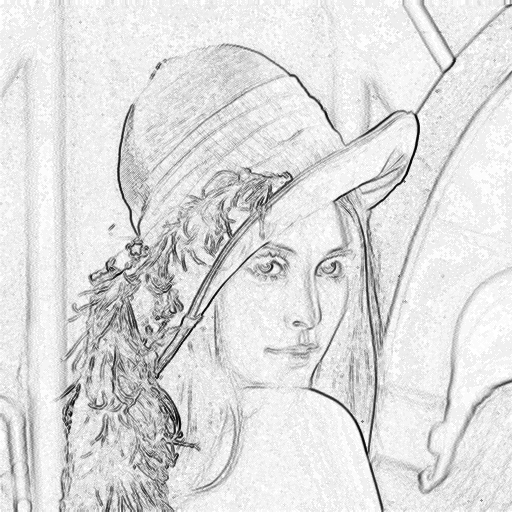
\includegraphics[width=.2\linewidth]{../figures/geninput-000b}}  &
    \fbox{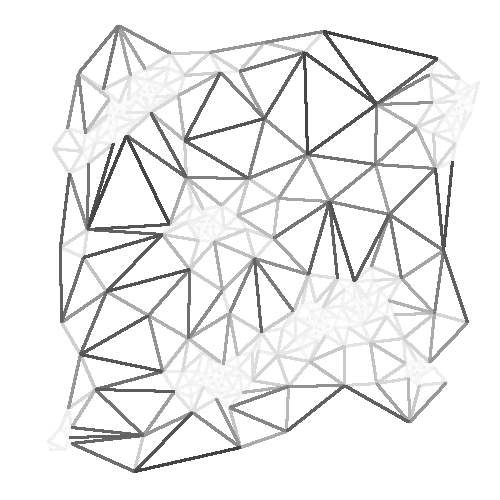
\includegraphics[width=.2\linewidth]{../figures/geninput-001b}}  &
    \fbox{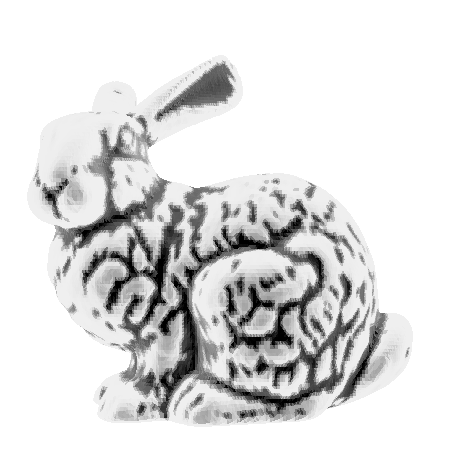
\includegraphics[width=.2\linewidth]{../figures/geninput-002b}}
    \\[5pt]
    %
    sortie:                                                                &
    \fbox{
\includegraphics[width=.2\linewidth]{../figures/genoutput-000}}  &
    \fbox{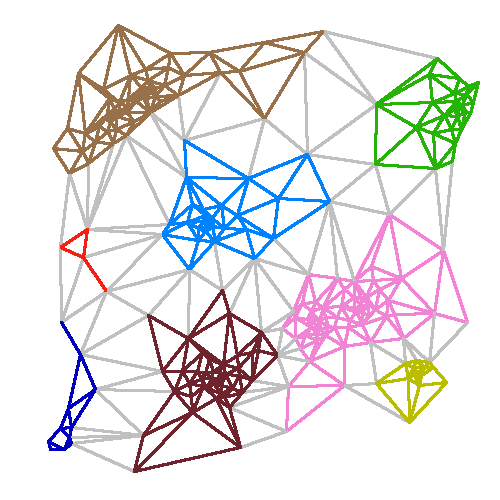
\includegraphics[width=.2\linewidth]{../figures/genoutput-001b}} &
    \fbox{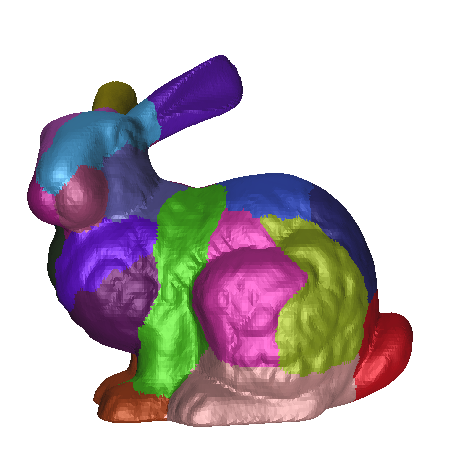
\includegraphics[width=.2\linewidth]{../figures/genoutput-002b}}
    \\
  \end{tabular}
  \bigskip

  \text{Le même code tourne sur toutes ces différentes données d'entrée.}

  \caption[]{Algorithme de ligne de partage des eaux appliqué à trois types d'image différents.}
  \label{resume:fig:type.vs.algo}
\end{figure}

La généricité peut avoir deux significations différentes selon les personnes à qui vous demandez. Par exemple, certaines
diront que la généricité est un aspect haut niveau et qualifie un outil << suffisamment générique >> pour gérer tous ses
cas d'utilisation. D'autres soutiendront que la généricité concerne la façon dont le code est écrit : suffisamment
générique pour gérer tous les cas d'utilisation possibles. Ni l'un ni l'autre n'a tort. Cependant, pour des raisons de
compréhension, nous utiliserons des mots différents pour chacun de ces cas. Un outil assez générique pour gérer un grand
nombre de cas d'utilisation sera appelé \emph{versatile}. Enfin, pour un outil dont le but est de fournir une un
environnement de programmation capable de gérer le code de n'importe quel cas d'utilisation, nous utiliserons le terme
\emph{généric}. Dans cette thèse, la généricité concernera le code. La~\cref{resume:fig:type.vs.algo} illustre ce
résultat de la même implémentation générique de l'algorithme de ligne de partage des eaux appliqué sur une image 2D, un
graphe ainsi qu'un maillage.

Dans ce chapitre nous présentons l'origine de la programmation générique, qui remonte
jusqu'à~\citedate[année]{musser.1988.generic} et comment elle a évolué pour être intégrée dans le langage de
programmation Ada puis dans le langage de programmation C++. Ensuite, elle a encore évolué avec la notion de
\emph{concept} qui complétera la boîte à outils nécessaire pour pouvoir pleinement utiliser la programmation générique
sans recourir à des techniques et outils obscurs.

\begin{table}[htbp]
  \centering
  \begin{threeparttable}
    \caption[]{Approches de la généricité: avantages ~\& inconvénients}
    \begin{tabular}[width=0.8\linewidth]{l|ccccc}
      Paradigme                     & VT\tnote{1} & SC\tnote{2} & E\tnote{3} & Une IA\tnote{4} & AE\tnote{5} \\
      \hline
      Duplication de Code           & \cmark      & \xmark      & \cmark     & \xmark          & \xmark      \\
      Généralisation de Code        & \xmark      & \eqmark     & \eqmark    & \cmark          & \xmark      \\
      Programmation Orientée Object & \eqmark     & \cmark      & \xmark     & \cmark          & \cmark      \\
      Programmation Générique:      &             &             &            &                 &             \\
      \quad avec C++11              & \cmark      & \eqmark     & \cmark     & \cmark          & \eqmark     \\
      \quad avec C++17              & \cmark      & \cmark      & \cmark     & \cmark          & \eqmark     \\
      \quad avec C++20              & \cmark      & \cmark      & \cmark     & \cmark          & \cmark      \\
    \end{tabular}
    \begin{tablenotes}
      \item[1] VT: vérification de type.
      \item[2] SC: simplicité du code.
      \item[3] E: efficacité.
      \item[4] Une IA: une seule implémentation par algorithme.
      \item[4] AE: abstraction explicite / généricité contrainte.
    \end{tablenotes}
    \label{resume:table:gen.approaches}
  \end{threeparttable}
\end{table}

Ce chapitre explore les possibilités de réaliser de la programmation générique au sein d'une bibliothèque. En effet, il
y a trois techniques permettant à l'utilisateur d'écrire une seule fois un algorithme de haut niveau pouvant s'exécuter
sur tous les types. Elles sont les approches de \emph{duplication de code}, de \emph{généralisation} et de
\emph{polymorphisme d'inclusion et paramétrique}~\parencite{gibbons.2007.datatype}. Nous présentons dans
la~\cref{resume:table:gen.approaches} le résultat de la comparaison de ces approches par rapport aux aspects qui nous
intéressent. Nous abordons également les limitations liées à l'utilisation de ces approches en comparant OpenCV,
Scikit-image et Pylene qui utilisent les quatre techniques à différents niveaux pour atteindre différents objectifs de
généricité, de performance et de facilité d'utilisation. De plus, nous avons identifié des limites liées au type de
données sous-jacent, à la structure du domaine et aux optimisations sur lesquelles nous discuterons des performances via
un benchmark concret.

Ce chapitre explore également comment la programmation générique est gérée dans les langages de programmation. Nous
retraçons comment Ada l'a implémenté, et ensuite comment C++ a permis l'expression de clauses contraintes \emph{require}
(concept) dès C++98, même si c'était relativement limitée à cette époque. Nous explorons comment les techniques de
métaprogrammation se sont développées et ont évoluées, en même temps que langage de programmation C++ lui-même, pour
enfin atteindre un point en 2020 (C++20) où il est possible d'écrire des concepts en C++.

Enfin, ce chapitre présente la limitation inhérente aux templates C++, à savoir qu'ils restent dans le monde statique
(moment de la compilation). La généricité (au sens concept C++) n'existe pas dans le binaire final livré à
l'utilisateur. L'utilisateur final, dans son monde dynamique (moment de l'exécution) ne peut pas utiliser un outil
générique (code C++). Nous discutons des différentes approches possibles pour combler cet écart entre le monde statique
(à la compilation) et dynamique (à l'exécution).

Le chapitre suivant fera un large usage de la généricité pour présenter la première contribution de cette thèse : une
taxonomie des concepts liés au traitement d'images.


\subsection*{Taxonomie pour le traitement d'images : types d'images et algorithmes}


Dans cette thèse, nous avons recherché la meilleure façon d'appliquer les nouvelles fonctionnalités génériques du
langage C++ dans le domaine du traitement d'image. Cela nous permet de les tester de manière pratique sur notre zone de
prédilection tout en nous souvenant de nos travail passé, à la fois les succès et les échecs en la matière. Cependant,
comme nous l'avons vu dans le chapitre précédent (Programmation générique (généricité)), faire naître des concepts à
partir due code est quelque chose qui se fait de manière émergente. Désormais, les premiers travaux seront de faire un
inventaire de tous les algorithmes d'images existants ainsi que de tous les algorithmes de traitement d'images (les deux
basiques et plus complexes) auxquels nous pouvons penser. De cette façon, nous remarquerons des modèles de comportement
émergeant de types d'images similaires ou algorithmes similaires. Nous pourrons alors extraire des schémas
comportementaux de cet inventaire afin de produire une taxonomie complète sous la forme d'un environnement constitué de
concepts liés au traitement d'images. Ce chapitre est structuré comme suit. Dans un premier temps, nous étudierons
comment extraire un schéma comportemental d'un algorithme simple afin de l'affiner en un ou plusieurs concepts. Dans un
second temps nous étudierons la théorie des ensembles de types d'images, leurs conjonctions et disjonctions. Nous
produirons également un inventaire des algorithmes de traitement d'images limité à la morphologies mathématiques que
nous pouvons exploiter pour l'étape finale. Troisièmement, nous étudierons la généricité intrinsèque des algorithmes
pour produire des canevas tirant parti des propriétés (liées aux types). Enfin, nous étudierons les schémas
comportementaux, relatifs à l'inventaire pré-établi des algorithmes, sous la forme d'une taxonomie inscrite dans un
environnement de concepts relatifs au traitement d'images.

Dans ce chapitre, nous présentons que les concepts ne sont pas conçus d'après des structures de données mais d'après des
algorithmes. En effet, un concept consiste à extraire un schéma comportemental cohérent d'un bout de code (algorithme)
et à le nommer pour lui donner une signification. A travers un exemple simple mais concret, nous présentons de manière
didactique comment extraire des concepts d'un algorithme de traitement d'image (correction gamma).

\begin{figure}[htbp]
  \centering
  \subfloat[Differentes versions de l'algorithm \emph{fill} ]{
    \includegraphics[width=1.9in]{../figures/image_version}
  }%
  \hfil
  \subfloat[Specialisation existant au sein d'une version]{
    \includegraphics[width=2.9in]{../figures/image_version_specialization}
  }%
  \caption[]{Ensemble des versions d'algorithme (a) et de ses spécialisations existant au sein d'une version (b).}
  \label{resume:fig:image.version.vs.specialization}
\end{figure}

Ce chapitre explique ensuite comment, en théorie, les types d'images sont reliés les uns aux autres. Nous présentons
l'ensemble de différents types d'images et comment les algorithmes existent dans ces ensembles, ce qui introduit la
notion de \emph{version} d'un algorithme. Un algorithme aura différentes \emph{versions} pour chaque ensemble de types
d'images qu'il prend en charge. Nous le distinguons (in~\cref{resume:fig:image.version.vs.specialization}) des
\emph{spécialisation} d'algorithmes, cette dernière étant la possibilité de profiter d'une opportunité (liée à une
propriété) pour faire une optimisation et augmenter les performances.

Ce chapitre décrit ensuite la notion de canevas d'algorithme qui est le résultat découlant de la taxonomie des
algorithmes de traitement d'images. En effet, il existe trois grandes familles d'algorithmes : les algorithmes
fonctionnant pixel par pixel (binarisation), les algorithmes locaux (dilatation) et les algorithmes globaux (Chamfer
distance transform). Nous nous concentrons principalement sur les algorithmes locaux et comment ils peuvent tous être
écrits à travers le même canevas de code. En effet, par exemple, la seule différence entre une dilatation et une érosion
est l'opérateur (max \vs min). Nous discutons ensuite des possibilités offertes par l'exploitation de ces canevas pour
possiblement résoudre des problèmes informatiques hétérogènes.

\begin{figure}[htbp]
  \centering
  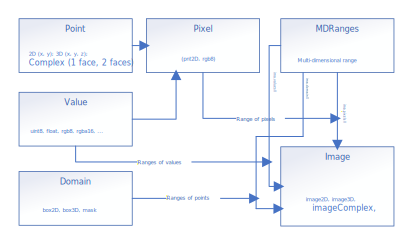
\includegraphics[width=.8\linewidth]{../figures/concepts/image}
  \caption[]{Concept Image.}
  \label{resume:fig:concept.image}
\end{figure}

Enfin, ce chapitre introduit notre première contribution principale : une taxonomie complète relative au domaine du
traitement d'image. Nous introduisons d'abord des concepts fondamentaux tels que \emph{point}, \emph{pixel},
\emph{domaine} et \emph{image} (illustrés dans la~\cref{resume:fig:concept.image}). Nous motivons et introduisons
ensuite des concepts avancés liés aux images et aux différentes manières d'accéder aux données (parcours en avant,
renversé, indexation, accès direct à la mémoire tampon sous-jacente, \ ldots). En fin de compte, nous introduisons les
concepts liés aux notions gravitant autour le traitement d'image, telles que les \emph{éléments structurant}, les
\emph{voisinages} et les \emph{extensions} (gestion des bordures) qui sont nécessaires pour pouvoir travailler avec des
algorithmes locaux.

Le chapitre suivant utilisera les concepts présentés pour introduire la deuxième contribution principale de cette thèse
: les \emph{vues d'images}.


\subsection*{Les Vues d'Image}


Cette notion de vues n'est pas nouvelle~\parencite{novak.1997.reuse} et est apparue naturellement en Traitement d'image
avec Milena~\parencite{geraud.2012.ipolmeeting,levillain.2010.icip} sous le nom de
\emph{morpher}~\parencite{levillain.2009.ismm, geraud.2012.hdr}. Il était toujours utile de pouvoir projeter une image à
travers un prisme qui pourrait extraire des informations spécifiques à son sujet sans avoir besoin de copier la mémoire
tampon des données sous-jacentes. Aujourd'hui (2020), le langage C++ (norme 20) introduit aussi ce mécanisme avec les
ranges~\parencite{niebler.2014.ranges} pour les \emph{collections non-propriétaire} (de leur mémoire). Il est nommé
\emph{vues} (view) et permet à l'utilisateur d'accéder au contenu d'un conteneur (vector, map) à travers un prisme. Dans
Pylene, nous avons décidé de nous aligner avec la nomenclature décidée dans C++20 afin de ne pas dérouter l'utilisateur.
De cette façon, une vue \texttt{transform} dans le traitement d'image fera la même chose sur une image que ce que la vue
\texttt{transform} fait sur un conteneur (collection) dans la bibliothèque de ranges standard. Les \emph{vues}
présentent les propriétés suivantes : \emph{copie quasi-gratuite}, \emph{non-propriétaire} (ne \emph{possède} aucune
tampon mémoire contenant des données), \emph{évaluation paresseuse} (l'accès à la valeur d'un pixel peut nécessiter des
calculs) et \emph{compositable}. Lorsque les vues sont chaînées, le compilateur construit un \emph{arbre d'expressions}
(ou \emph{expression template} tel qu'utilisé dans de nombreuses bibliothèques de calcul scientifique telles que as
Eigen~\parencite{guennebaud.2010.eigen}), il connaît donc à la compilation le type de la composition finale et s'assure
qu'il n'y ait pas de surcoût en performance à l'execution (0-overhead). Tout d'abord nous motivons l'utilisation des
\emph{vues} dans le traitement d'image, ensuite nous présentons les principales vues utilisées en traitement d'images.
Enfin, nous discuterons de la façon dont les vues d'image diffèrent de celles utilisées dans les ranges de C++ et leurs
principales propriétés (en particulier comment elles conservent/suppriment les propriétés de l'image parente) à travers
un exemple concret : la gestion des bordures et des extensions. Enfin, nous discuterons des limites lées à ce design.

En traitement d'images, un algorithme s'écrit naïvement en prenant une ou plusieurs données d'entrée (parmis lesquelles
figure la/les image(s) d'entrée), en effectuant un traitement sur ces données d'entrée puis en retournant les données
résultantes (ou une erreur). Prenons par exemple l'exemple de l'algorithme mélange alpha (alpha-blending) qui peut être
implémenté en C++ naïf comme suit :
\begin{minted}{C++}
  void blend_inplace(const uint8_t* ima1, uint8_t* ima2, float alpha,
  int width, int height, int stride1, int stride2) {
    for (int y = 0; y < height; ++y) {
      const uint8_t* iptr = ima1 + y * stride1;
      uint8_t* optr = ima2 + y * stride2;
      for (int x = 0; x < width; ++x)
        optr[x] = iptr[x] * alpha + optr[x] * (1-alpha);
    }
  }
\end{minted}

Ce code a plusieurs défauts. Il fait des hypothèses fortes sur les images d'entrée : la contiguïté de ses données dans
sa mémoire tampon et sa forme (2D). Supposons que notre utilisateur veuille maintenant restreindre l'algorithme à une
région spécifique à l'intérieur de l'image. Le mainteneur devrait alors fournir une surcharge de fonction pour
l'algorithme avec un argument d'entrée supplémentaire correspondant à la région d'intérêt. Supposons que l'utilisateur
veuille maintenant prendre en charge la manipulation d'images 3D. Le mainteneur devrait maintenant fournir fournir deux
surcharges de fonction supplémentaires avec un argument de \emph{pas} supplémentaire (un pour l'algorithme de base, un
l'algorithme prenant en compte une région d'intérêt). Supposons maintenant que l'utilisateur souhaite uniquement
manipuler le canal de couleur rouge. Maintenant le mainteneur doit prendre en charge et ajouter des surcharges de
fonctions supplémentaires pour chaque canal et/ou type de couleur. La complexité augmente grandement pour chaque points
de customisation que le mainteneur souhaite offrir à l'utilisateur. Bien sûr, il est possible d'empêcher la duplication
de code grâce à une utilisation intelligente des techniques d'ingénierie informatique (factorisation de code, etc.) mais
la complexité fuiterait toujours à travers l'API dans une certaine mesure. C'est ainsi que l'autre solution consiste à
permettre à l'utilisateur de effectuer ces restrictions en amont de l'algorithme de manière transparente afin que
l'algorithme en aval soit facile à écrire, comprendre et maintenir. Pour y parvenir, nous devons augmenter le niveau
d'abstraction autour des images d'un niveau afin que nous puissions travailler au directement niveau de l'image.
L'algorithme de mélange alpha (alpha-blending) s'écrirait alors comme indiqué dans la~\cref{resume:fig:view.alphablend}.

\begin{figure}[htbp]
  \centering
  \includestandalone[mode=image, scale=0.7]{../figures/alphablend}

  \caption[]{Algorithme mélange alpha (alpha-blending) écrit a niveau de l'image.}
  \label{resume:fig:view.alphablend}
\end{figure}

Cette façon d'exprimer un algorithme est obtenue en introduisant des \emph{vues} dans le traitement d'image. Une image
est maintenant une vue et peut être restreinte/projetée/manipulée selon les besoins de l'utilisateur avant de la
transmettre à un algorithme. Même l'algorithme de mélange alpha (alpha-blending) peut entièrement être réécrit en termes
de vues, comme montré dans ~\cref{resume:fig:new.alphablend}.

\begin{figure}[htbp]
  \centering
  \begin{minipage}[b]{5.5cm}
    \includestandalone[mode=image, scale=1.0]{../figures/view_ast2}
  \end{minipage}
  \begin{minipage}[b]{5.5cm}
    \begin{minted}{c++}
    auto alphablend =
      [](auto ima1, auto ima2, float alpha) {
        return alpha * ima1 + (1 - alpha) * ima2;
      };
    \end{minted}
    \bigskip
    \bigskip
    \bigskip
  \end{minipage}
  \caption[]{Mélange alpha (alpha-blending), implementation générique avec les \emph{views}, et son arbre d'expression.}
  \label{resume:fig:new.alphablend}
\end{figure}

Être capable d'effectuer de puissantes manipulations sur les images avant de les passer aux algorithmes annule
complètement le problème initale qui consiste à avoir plusieurs surcharge de fonctions pour un même algorithme tout en
maintenant et en documentant toutes les arguments optionnels associés. En effet, pour effectuer la transformation de
mélange alpha (alpha-blending) sur l'image d'entrée, tout ce que l'utilisateur doit faire est :
\begin{minted}{C++}
  auto ima1, ima2 = /* ... */;
  auto ima_blended = alphablend(ima1, ima2, 0.2);
\end{minted}
Si l'utilisateur souhaite restreindre la région à mélanger ou le canal de couleur sur lequel travailler, il lui suffit
d'écrire le modification suivante :
\begin{minted}{C++}
  auto roi = /* ... */;
  auto blended_roi = alphablend(view::clip(ima1, roi), view::clip(ima2, roi), 0.2);
  auto blended_red = alphablend(view::red(ima1), view::red(ima2), 0.2);
\end{minted}
La restriction est faite en amont de l'algorithme et propagée en aval sans augmenter la complexité du code. De cette
façon, la vue augmente considérablement ce que l'utilisateur peut faire tout en écrivant moins de code.

\begin{figure}[htbp]
  \centering
  \includegraphics[scale=0.7]{../figures/pipeline}
  \caption[]{Exemple d'une pipeline de traitement d'image simple.}
  \label{resume:fig:view.pipeline}
\end{figure}

Dans ce chapitre, nous voyons que \emph{les vues sont composables}. L'une des caractéristiques les plus importantes dans
la conception d'une pipeline (généralement, en génie logiciel) est la \emph{composition d'objets}. Elle permet de
composer des blocs simples en blocs complexes. Ces blocs complexes peuvent alors être gérés comme s'il s'agissait encore
de blocs simples. Dans~\cref{resume:fig:view.pipeline}, nous avons 3 opérateurs d'image simples
\emph{Image}~\(\rightarrow\)~\emph{Image} (la conversion en niveaux de gris, la sous-quantification et la dilatation).
Comme indiqué dans la~\cref{resume:fig:view.comp}, la composition de l'algorithme considérerait ces 3 opérateurs simples
comme un seul opérateur complexe \emph{Image}~\(\rightarrow\)~\emph{Image} qui pourrait ensuite être utilisé dans un
autre encore plus complexe pipeline de traitement. Tout comme les algorithmes, les vues d'image sont composables, \prex,
une vue de la vue d'une image est toujours un image. Dans ~\cref{resume:fig:view.comp}, nous composons l'image d'entrée
avec une vue de transformation en niveaux de gris et une vue de sous-quantification qui alimente ensuite l'algorithme de
dilatation.

\begin{figure}[htbp]
  \centering
  \includegraphics[scale=0.7]{../figures/composition}
  \caption[]{Exemple d'une pipeline de traitement d'image simple illustrant la différence entre la composition
    d'algorithmes et la composition de vues d'image.}
  \label{resume:fig:view.comp}
\end{figure}

Aussi, les \emph{vues améliorent l'utilisabilité}. Le code pour composer des images dans ~\cref{resume:fig:view.comp}
est presque aussi simple que :

\begin{minted}{c++}
  auto input = imread(...);
  auto A = transform(input, [](rgb16 x) -> float {
    return (x.r + x.g + x.b) / 3.f; }; );
  auto MyComplexImage = transform(A, [](float x)
    -> uint8_t { return (x / 256 + .5f); }; );
\end{minted}

Les personnes familiarisées avec la programmation fonctionnelle peuvent remarquer des similitudes avec ces langages où
\emph{transform} (\emph{map}) et \emph{filter} sont des opérateurs de séquence. Les vues utilisent le paradigme
fonctionnel et sont créées par des fonctions qui prennent une fonction en argument : l'opérateur ou le prédicat à
appliquer pour chaque pixel ; nous n'itérons pas à la main sur les pixels de l'image.

De plus, les \emph{vues améliorent la ré-utilisabilité}. Les extraits de code ci-dessus sont simples mais peu
réutilisables. Cependant, suivant le paradigme de la programmation fonctionnelle, il est assez facile de définir de
nouvelles vues, car certains adaptateurs d'image peuvent être considérées comme des \emph{fonctions d'ordre supérieur}
pour lesquelles on peut lier certains paramètres, comme on le ferait avec la technique de
currying~\parencite{hanus.1995.curry}. Dans~\cref{resume:fig:view.highorder}, nous montrons comment la primitive
\emph{transform} peut être utilisée pour créer une vue additionnant deux images et un opérateur de vue effectuant la
conversion en niveaux de gris ainsi que la sous-quantification réutilisable par la suite\footnote{Ces fonctions auraient
  pu être écrites de manière plus générique pour plus de ré-utilisabilité, mais ce n'est pas le but ici.}.

\begin{figure}
  \begin{minted}{c++}
auto operator+(Image A, Image B) {
  return transform(A, B, std::plus<>());
}
auto togray = [](Image A) { return transform(A, [](auto x)
  { return (x.r + x.g + x.b) / 3.f; };)
};
auto subquantize16to8b = [](Image A) { return transform(A,
  [](float x) { return uint8_t(x / 256 +.5f); });
};

auto input = imread(...);
auto MyComplexImage = subquantize16to8b(togray(A));
  \end{minted}

  \caption[]{Utilisation de fonctions d'ordre supérieur pour créer des opérateurs de vues personnalisées.}
  \label{resume:fig:view.highorder}
\end{figure}

De plus, \emph{les vues sont calculées paresseusement}. L'opération étant enregistrée dans la vue d'image, ce nouveau
type d'image permet de mélanger des types d'images fondamentaux avec des algorithmes. Dans~\cref{fig:view.highorder}, la
création de vues n'implique aucun calcul en soi mais retarde plutôt le calcul jusqu'à ce que l'expression \texttt{v(p)}
soit invoqué. Parce que les vues peuvent être composées, l'évaluation peut être assez retardée. Les adaptateurs d'image
sont des \emph{expression template}~\parencite{veldhuizen.1995.expression, veldhuizen.2000.blitz} car ils enregistrent
les \emph{expressions} utilisées pour générer l'image en tant que paramètre template. Une vue représente en fait un
arbre d'expressions (\cref{fig:new.alphablend}).

\emph{Les vues sont efficaces}. Avec un design classique, chaque opération de la pipeline est implémentée << par
elle-même >>. Chaque opération nécessite que de la mémoire lui soit allouée pour l'image de sortie et, également, chaque
opération nécessite que l'image soit entièrement parcourue. Ce design est simple, flexible, composable, mais n'est pas
efficace ni terme en mémoire ni performance de calcul. Avec l'évaluation paresseuse, l'image n'est parcourue qu'une
seule fois (lorsque la dilatation est appliquée), ce qui a deux avantages. Premièrement, il n'y a pas d'images
intermédiaires, ce qui est très efficient en termes de mémoire. Deuxièmement, la traversée de l'image est plus rapide
grâce à une meilleure utilisation du cache mémoire, et effectue une traversée selective optimale. En effet, dans notre
exemple (\cref{resume:fig:view.pipeline}), le traitement d'un pixel RGB16 de l'algorithme de dilatation le convertit
directement en niveaux de gris, puis le sous-quantifie en 8 bits, et enfin le rend disponible pour l'algorithme de
dilatation. Il agit \emph{comme si} nous écrivions un opérateur optimal qui combinerait tous ces opérations. Cette
approche est quelque peu liée aux opérations de fusion du noyau disponibles dans certains HPC
spécifications~\parencite{openvx.2019} mais la fusion de vues est optimisée par le compilateur C++
seulement~\parencite{brown.2018.ranges}. L'aspect sélectif intervient lorsqu'une région d'intérêt intervient dans la
pipeline de traitement. En effet, l'intégralité de la pipeline n'est alors exécuté que sur la région d'intérêt et ce
même si cette sélection n'est faite qu'à la toute fin de la pipeline de traitement.

Enfin, les \emph{vues améliorent la productivité}. Tous les algorithmes de traitement d'image fonctionnant pixel par
pixel peuvent (et doivent) être réécrits intuitivement en utilisant une vue en une seule ligne. Les vues
\emph{transform} sont la clé permettant ce point. Cela implique qu'il existe un nouveau niveau d'abstraction disponible
pour le traiteur d'image lors du prototypage de son algorithme. Le temps passé à la mise en oeuvre des fonctionnalités
est réduite, donc le temps de la boucle de rétroaction est également réduit. Cela amène naturellement un gain de
productivité au traiteur d'image.


\subsection*{Un pont entre le monde statique et le monde dynamique}


Dans le monde de la programmation, il existe trois grandes familles de language de
programmation~\parencite{prechelt.2000.comparison}. Il existe (i) les langages de programmation \emph{compilés}, tels
que C, C++, Rust ou Go, (ii) les langages de programmation \emph{interprétés}, tels que Python, PHP, Lisp ou Javascript,
et (iii) les langages de programmation hybrides, tels que Java ou C\#. Ces derniers ont une passe de compilation rapide
qui compile le code source dans un bytecode intermédiaire. Ensuite, ce bytecode est interprété via un interpréteur sur
une machine hôte.

\begin{figure}[htbp]
  \centering
  \includegraphics[width=.6\linewidth]{../figures/type-erased_buffer}
  \caption[]{Pont entre Python et C++ grâce à Pybind11 et un effacement de type en C++.}
  \label{resume:fig:type-erased.buffer}
\end{figure}

Dans ce chapitre, nous concevons de nombreuses solutions pour résoudre plusieurs types de problèmes liés au pont entre
le montre statique et le monde dynamique. Nous présentons notre solution hybride capable de rendre disponible notre
bibliothèque générique C++ (statique) à partir de Python (dynamique). Nous discutons à propos des différentes façons de
réaliser ce pont, leurs avantages et leurs inconvénients. Aussi, nous introduisons une nouvelle couche d'abstraction, le
value-set, qui est un moyen standard de manipuler les valeurs sous-jacentes d'une image, utilisable lors de la mise en
oeuvre d'algorithmes de traitement d'images. Cette nouvelle couche d'abstraction permet notament à l'utilisateur
d'injecter du code côté Python dans des routines C++ déjà compilées. Cependant, superposer une couche d'abstraction
après l'autre, ou même appeler du code Python entraine forcément un coût du côté des performances. C'est pourquoi nous
avons réalisé un benchmark pour exposer clairement le coût de nos différentes solutions. Ce benchmark compare les quatre
versions de notre algorithme d'étirement (stretch) dont l'implémentation et l'utilisation sont détaillées dans le
chapitre. Le résultat est affiché dans le~\cref{resume:table:static.dynamic.perfs}.

\begin{table}[htbp]
  \footnotesize
  \centering
  \begin{tabular}{l|ccc}
    \toprule
    Dispatch type                                                                                            &
    Compute Time                                                                                             &
    \(\Delta{}\)Compute Time
    \\ \midrule Value-set natif avec des types de valeurs C++ natifs (baseline)
                                                                                                             & \(0.0093s\) & \(0\) \\
    Value-set comprenant un appel virtuel avec des types de valeurs C++ natifs                               &
    \(0.1213s\)                                                                                              &
    \(\times 13\)
    \\
    Value-set comprenant un appel virtuel avec des types de valeurs C++ en cachées par un effacement de type &
    \(1.0738s\)                                                                                              &
    \(\times 115\)
    \\
    Value-set injecté depuis Python ave Python avec des types de valeurs C++ natifs                          &
    \(21.5444s\)                                                                                             &
    \(\times 2316\)
    \\
    \bottomrule
  \end{tabular}
  \caption[]{Benchmarks de toutes nos version de l'algorithme d'étirement (stretch).}
  \label{resume:table:static.dynamic.perfs}
\end{table}

Ce benchmark montre que chaque fois qu'une couche d'abstraction est ajoutée au-dessus de baseline, l'utilisateur doit
s'attendre à un facteur \(10\times\) impactant les performances de son code. De plus, appeler du code Python est
immensément plus lent (\(2300\times\) !) que la baseline. Cela renouvelle l'intérêt de recompiler la bibliothèque C++
générique avec avec un type paramétrique supplémentaire connu plutôt que de l'injecter depuis Python, surtout pour du
code qui met longtemps à s'exécuter. Pouvoir injecter du code Python facilite le prototypage et augmenter la vitesse à
laquelle l'utilisateur peut écrire son code. Cependant, le benchmark montre que ce n'est pas une solution viable une
fois que le prototype doit être déployé dans un environnement de production.

\paragraph{Continuité : Solutions basées sur le JIT, avantages et inconvénients}

Notre solution hybride a certainement des avantages, mais l'énorme inconvénient est la lenteur à injecter nos propres
types à partir de le côté Python. Il existe une autre solution que cette thèse n'a pas eu l'occasion d'approfondir. Ce
solution est basée sur une technologie connue : la compilation Just-In-Time (JIT) qui a été illustrée précédemment
in~\cref{fig:static.dynamic.dynamic.pipeline} (et qui lui-même repose sur la notion de générative
programmation~\parencite{czarnecki.2000.generative}). Des bibliothèques telles que
AsmJit~\parencite{kobalicek.2011.asmjit} sont capables de émettre du code machine directement en effectuant un appel en
code C++. En effet, c'est une technologie déjà utilisée par les langages interprétés tels que Java ou PHP pour générer à
la volée du code machine natif et optimisé pour la section du code source qui est considéré comme "chaud" par
l'interprète. Un code source est ``chaud'' lorsqu'il est beaucoup exécuté : l'utilisateur final gagnerait payer le temps
de compilation une fois pour que ce code soit exécuté plus rapidement plusieurs fois par la suite. Lors de l'application
de cette stratégie à notre problématique, cela signifierait que l'utilisateur doit être capable de compiler du code
machine natif à partir du modèle générique Le code C++ injecte le type demandé lorsqu'il est utilisé. Une telle
opération déplace fortement la charge sur l'utilisateur, et il est bien connu que compiler du code C++ est notamment
\emph{compliqué} et \emph{lent}. De plus, la bibliothèque doit être capable de générer automatiquement la liaison Python
une fois le code compilé. Il existe plusieurs solutions pour réaliser ce procédé.

La première solution consiste essentiellement à utiliser l'appel système aux compilateurs pour réellement
\emph{compiler} le code C++ une fois que le les types modélisés sont connus et explicitement instanciés dans le code
source. Cette solution nécessite une génération de code minutieuse conception et que l'utilisateur possède effectivement
un compilateur sur son ordinateur. De plus, l'utilisateur doit résoudre tous les dépendances de bibliothèque, telles que
\emph{freeimage} pour IO, etc. Cette solution a été conçue dans le VCSN bibliothèque~\parencite{demaille.2013.vcsn}. En
effet, à chaque fois que l'utilisateur déclare un nouvel automate dans son notebook Jupyter, le code source
correspondant est compilé au premier plan puis mis en cache. C'est une solution très périlleuse à mettre en place
lorsque l'environnement d'exécution final (OS, logiciels installés) n'est pas bien connu à l'avance. De nos jours, le
problème peut être moindre, cependant, il nécessite toujours de maintenir à la fois la bibliothèque et la solution de
conteneur pour l'utiliser.

La troisième solution consiste à s'appuyer sur des projets récents qui reposent tous sur l'infrastructure LLVM. Nous
pouvons notez notamment AutoWIG~\parencite{fernique.2018.autowig}, Cppyy~\parencite{wimtlplavrijsen.2016.cppyy},
Xeus-cling~\parencite{quantstack.2021.xeus-cling} et Pythran~\parencite{guelton.2015.pythran}. AutoWIG a en interne code
basé sur LLVM/Clang pour analyser le code C++ afin de générer et compiler une liaison Swig Python à l'aide de Mako
moteur de template. AutoWIG, couplé à Cython permettrait à l'utilisateur, par exemple, de générer du code C lié à un
structure Python personnalisée. Ensuite, un simple appel à AutoWIG analysera le code C et l'injectera dans la
bibliothèque C++ pour générer les liaisons appropriées pour l'utilisateur. Quant à Cppyy, il est basé sur LLVM/Cling, un
interpréteur C++, et peut interpréter directement le code C++ à partir d'une chaîne Python. Cela permet d'injecter
facilement des types personnalisés, qu'ils soient dans du code Python (transpilé avec Cython) ou du code C++
(directement interprété par Cling). Ensuite, l'infrastructure génère le liaison appropriée à partir de la bibliothèque
C++ basée sur un modèle pour le type injecté. Xeus-cling est un noyau Jupyter prêt à l'emploi et permettre l'utilisation
du code C++ directement à partir d'un bloc-notes. Cela contourne complètement le besoin d'une liaison Python dans la
première place et permettre à l'utilisateur d'utiliser la bibliothèque depuis le bloc-notes comme s'il utilisait une
bibliothèque Python. Enfin, Pythran est un compilateur avancé pour un sous-ensemble du langage Python, axé sur le calcul
scientifique. Il prend un modèle Python annoté avec quelques descriptions d'interface et le transforme en un module
Python natif avec le même interface, mais j'espère plus rapide. Pythran tire parti des instructions multicœurs et SIMD
pour transformer son sous-ensemble de le langage Python en code C++ fortement modélisé instancié pour des types
optimisés particuliers. Tous ceux les infrastructures, cependant, ont un coût élevé en termes de taille binaire. En
effet, un compilateur C++ n'est pas petit et l'embarquer avec la bibliothèque de traitement d'image peut facilement
avoir un impact considérable sur le binaire final. Sans le LLVM infrastructure, le binaire peut peser environ 3 Mo. Avec
l'infrastructure LLVM, le poids binaire au strict minimum 50 Mo. De plus, ces solutions peuvent ne pas être
immédiatement plus rapides. En effet, lors du prototypage aller-retour avec une variété de types, l'utilisateur peut ne
pas être impatient d'attendre de longues compilations à chaque fois qu'il teste avec une nouvelle itération de son
travailler. Malgré ces faits, ces solutions offrent une excellente voie de recherche pour l'avenir et l'auteur est
impatient de enfiler ces chemins.


\subsection*{Conclusion}


Le travail présenté dans cette thèse par l'auteur a suivi un arc narratif très clair. L'accent a d'abord été mis sur
présenter ce qu'est la notion de programmation générique (généricité), son histoire et comment chacun peut se rapporter
à son quotidien utilisation, en particulier lorsqu'elle est appliquée au traitement d'images. La généricité est une
notion vieille de 4 décennies qui a évolué et trouvé une utilisation dans un domaine très moderne de notre société. En
particulier, dans le traitement d'images, il est largement utilisé pour construire des applications utilisées dans le
monde entier. Cependant, il a été démontré à quel point il peut être difficile de mettre en œuvre des solutions reposant
sur la généricité. En effet, il existe une règle de trois liant généricité, performance et facilité d'utilisation. La
règle stipule qu'on ne peut avoir que deux de ces objets en sacrifiant le troisième. Si l'on veut être générique et
efficace, alors la solution naïve sera très complexe à utiliser avec beaucoup de paramètres. Si l'on veut qu'une
solution soit générique et facile à utiliser, alors ce ne sera pas très efficace par défaut. Enfin, si l'on veut une
solution simple d'utilisation et efficace alors ce ne sera pas très générique. Dans cette thèse, nous essayons de
démontrer comment briser cette règle en trois étapes.

La première étape, illustrée dans le chapitre \emph{Taxonomy for Image Processing}, consistait à faire un inventaire des
types d'images et familles ainsi que différents algorithmes de traitement d'images. L'objectif était de produire une
taxonomie complète des types (pixel, image, éléments structurants, \ldots) et algorithmes liés au traitement d'image
afin de pouvoir écrire concepts (au sens des concepts C++). Cette première étape délimite le périmètre de ce que
l'auteur entend par \emph{généricité}. A partir de ce point de départ, il devient plus facile d'écrire des algorithmes
de traitement d'image par défaut, juste en en s'appuyant sur ces concepts. De plus, différents concepts existent pour
permettre aux implémenteurs d'algorithmes d'exploiter les propriétés (décomposabilité des éléments structurants,
contiguïté du buffer de l'image, \ldots) afin d'atteindre des performances maximales.

A ce stade, on raisonne encore à un niveau bas (pixel) ce qui génère le besoin de concevoir une couche d'abstraction
dans afin de permettre un prototypage rapide pour des opérations simples tout en garantissant une empreinte mémoire très
faible et proche de zéro impact sur les performances. Pour cette raison, nous étendons le concept de \emph{vues} du
standard C++ (2020) aux images et concevoir ce que la notion de \emph{vue d'image}. Nous faisons également le choix de
conception d'avoir une image bon marché à copier (données partagées buffer) par défaut afin de fusionner l'image
concrète et les vues du point de vue de l'utilisateur. L'évaluation paresseuse, qui se produit systématiquement lorsque
l'utilisation des vues permet un gain de performances lors du découpage d'images volumineuses. Dans le cas où l'ensemble
l'image est traitée, nous avons pu tout de même retenir des performances très satisfaisantes qui restent stables. Aussi,
nous montrons à travers cas d'utilisation concrets, tels que l'algorithme pixel par pixel et la gestion des frontières
comment l'utilisation des vues simplifie grandement comment écrire des algorithmes de traitement d'image plus complexes
et efficaces par défaut. Nous montrons enfin les limites de cette approche, avec un accent particulier sur la vitesse de
parcours d'une image, un cas d'utilisation obligatoire que nous devons maîtriser.

Enfin, cette thèse a porté son attention sur la manière dont il est possible de distribuer ce logiciel au traitement
d'image communauté qui travaille principalement avec Python. Le dernier ouvrage concentre ses efforts sur la recherche
de la meilleure façon de concevoir un pont statique (compile-time, templated C++) --- dynamique (runtime, Python
notebook) pour apporter ces notions (concepts et vues) au praticien, efficacement. Ce dernier ouvrage explore ce dilemme
et propose de l'aborder avec une solution hybride dont la conception est expliquée en profondeur. Cette solution hybride
s'appuie sur un type effacé qui offre compatibilité avec un \emph{NumPy.array}~\parencite{harris.2020.numpy}. Il est
alors capable de se lancer à l'intérieur d'un \(n \fois n\) répartiteur (dimension et type sous-jacent) dans un type C++
modélisé concret optimisé. Cette solution aussi expliquer comment écrire très simplement le code glue permettant
d'exposer en Python des algorithmes déjà existants (en C++) grâce à une mécanique de dispatch fortement inspirée du
standard C++ (\texttt{std::visit}, \texttt{std::variant}). le Le but de cette solution était de regrouper en un seul
endroit dans le code tous les types supportés dans les répartiteurs pour à des fins de maintenance ainsi qu'un travail
minimal exigeant de la part de l'implémenteur d'algorithmes pour exposer leurs algorithmes, tout cela tout en gardant
les performances natives. En effet, aucune copie superflue n'est effectuée grâce à \emph{pybind11} \emph{type-caster},
et une conversion est effectuée du type effacé vers le type natif. Tout le travail qui est fait dans l'algorithme est
effectué sur le type natif optimisé. Enfin, cette solution offre un moyen d'injecter Python personnalisé types dans la
bibliothèque à des fins de prototypage, grâce à une nouvelle couche d'abstraction, au prix de lourdes performances
perte. L'inconvénient de cette solution est évidemment le gonflement du code avec la taille binaire résultante qui
explose de façon exponentielle avec le nombre de types pris en charge multiplié par le nombre d'algorithmes multiplié
par le nombre d'autres données supportées (éléments structurants, label map, etc.)

Nous concluons cette thèse en proposant de nouvelles pistes de recherche autour du domaine de la compilation JIT pour
améliorer encore le pont entre le monde statique et le monde dynamique. L'auteur pense que cette piste mérite d'être
explorée, surtout avec la des outils existants déjà prometteurs (Xeus-cling, Cppyy, Cython, AutoWIG) afin de résoudre le
problème de gonflement du code. Nous serions ne compilez que ce dont l'utilisateur a besoin, mais le prix d'entrée peut
être de lier statiquement un interpréteur C++ (LLVM/cling?) binaire qui en soi le gonflerait grandement. Il peut être
possible, cependant, de se fier à l'ensemble du système de l'utilisateur infrastructure pour que la maintenance ne
distribue pas tout un interpréteur/compilateur C++ à côté de son image binaire de la bibliothèque de traitement. Il
s'agit encore d'un domaine de recherche nouveau et l'auteur souhaiterait vivement l'approfondir pour étudier ce qu'il
est possible de réaliser dès aujourd'hui avec ces outils pour la communauté du traitement d'images.

\clearpage

\appendix

% This allows for an additional line-breaking pass with the amount of
% "tolerable" white space per line increased by 1em.
% Needed for overfull hbox in bibliography
\emergencystretch=1em

\label{sec:references}
\printbibliography[heading=bibintoc,title={References}]


\end{document}
